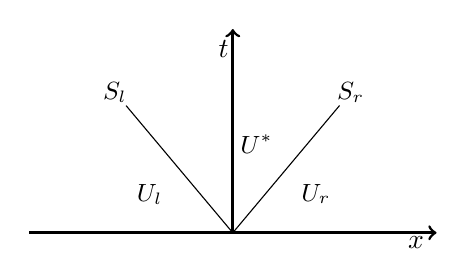
\begin{tikzpicture}[scale = {0.015\linewidth},inner sep = 1pt]
%% \begin{tikzpicture}[scale = {0.015\linewidth},inner sep = 1pt]
%% \tikzstyle{every node} = [draw,circle,fill=gray!30];
%% \draw (-1.5,0.0) circle (0.8);
%% \draw[<->,line width=1pt] (0,1) node[right]{\;$t$}|-(1,0) node[below]{$m$};
\draw[line width=1pt] (0,0.45) node[left]{$t$}|-(0.45,0) node[below]{$x$};
\draw[->,line width=1pt] (0.45,0)--(0.5,0); % extent x-axis  
\draw[->,line width=1pt] (0,0.45)--(0,0.5); % extent t-axis  
\draw[line width=1pt] (-0,0)--(-0.5,0); % draw negative x-axis  

\node[draw=white] (fr) at (-0.28925,0.34475) {\small $S_l$};
\node[draw=white] (fl) at (0.28925,0.34475) {\small $S_r$};

\node[draw=white] (Ul) at (-0.20392,0.095089) {\small $\mbf{U}_l$};
\node[draw=white] (Us) at (0.058234,0.21733) {\small $\mbf{U}^*$};
\node[draw=white] (Ur) at (0.20392,0.095089) {\small $\mbf{U}_r$};

%% \node[] at (0.15,0.95) {contact};
\draw (0,0) -- (fr);  
\draw (0,0) -- (fl);  
\end{tikzpicture}
